\section{Designing an Enjoyable Game}
\label{chap:design_an_enjoyable_game}

How to create an enjoyable game is an important part of every game development process. This chapter presents a literature study of the subject based on work conducted by \citeauthor{malone_what_1980} in 1980, and \citeauthor{sweetser_gameflow_2005}’s “GameFlow: a model for evaluating player enjoyment in games” article. \citeauthor{malone_what_1980}’s research outlines challenge, fantasy, and curiosity as the three main elements to increase motivation in games. The GameFlow article presents a model for evaluating enjoyment in games based on eight elements. Even though different authors wrote these articles, they present a lot of the same mindset in what characterizes an enjoyable game.

\subsection{What Makes Things Fun to Learn?}
Malone presented in his study from \citeyear{malone_what_1980} a framework for creating enjoyable games. As mentioned above, he organized the essential properties of what makes a good game into the three categories: challenge, fantasy, and curiosity. Malone wrote multiple articles on the topic. His main findings were summarized in “What Makes Things Fun to Learn? Heuristics for Designing Instructional Computer Games”. Even though this research was conducted in 1980 and the examples he presents are somewhat old, the main concepts are still highly relevant today.

\subsubsection{Challenge}
The first property presented by Malone is \textit{challenge}:

\begin{quote}\blockquote{\textit{In order for a computer game to be challenging, it must provide a goal whose attainment is uncertain.}} \citep{malone_what_1980}.\end{quote}  

From this principle, three essential characteristics of why challenge is necessary to create good computer games follow:

\textbf{Goal} \\
Based on studies done by Malone, users tend to prefer games that have clearly defined goals. However, it is necessary to note that all goals are not equally valuable. Consequently, four different properties on how to create appropriate goals are mentioned:

\begin{enumerate}
    \item Simple games should include obvious goals.
    \item A complex environment should provide a structure so that players can easily generate appropriately difficult goals.
    \item Practical and fantasy goals are often the best ones.
    \item Players need to know when they are getting closer to the goal.
\end{enumerate}

\textbf{Uncertain outcome} \\
The next characteristic is \textit{uncertain outcome}, and the article describes four different ways  it can make computer games more challenging:

\begin{enumerate}
    \item \textbf{Variable difficulty levels}\\ 
    Good computer games should include variable difficulty levels that can match the user’s skill level. The difficulty level can be determined in three ways: Automatically, chosen by the player, or determined by the opponent’s skills.
    \item \textbf{Multiple level goals} \\ 
    Finding a goal for various player types is easier when creating multiple-level goals. Generally, two levels of goals are defined: Basic goals and meta goals. One typical example of this could be to have a basic goal of completing platform game levels. Collecting all the coins could then be the meta-goal. 
    \item \textbf{Hidden information} \\
    Hiding information can be an appropriate way of creating challenging games. Guessing games use this technique regularly.
    \item \textbf{Randomness} \\
    One last way of creating challenging games is to include randomness. When a random element is included, the player cannot predict the next step, making the game more challenging. Gambling games primarily succeed based on using randomness.
\end{enumerate}

\textbf{Self-esteem} \\
In addition to goals and uncertain outcomes, self-esteem is mentioned in the article. Self-esteem can be seen as the reason why goals and challenges are essential in good games. Completing goals and challenges can increase a person’s self-esteem and thus create a captivating game.

\subsubsection{Fantasy}
The next property is fantasy, which is often used in games to make them more appealing. In games, fantasies often appear as models of physical objects and social settings that are not truly present \citep{malone_what_1980-1}.

One typical example where fantasy is used to increase enjoyment is in learning games, where one can increase the level of fun by overlaying the curriculum with elements of fantasy. The fantasy can visualize the progression of the player towards the goal based on right or wrong answers. An example could be getting to the finish line in a marathon or avoiding a catastrophe, like in Hangman. In these games, the fantasy depends on how the skill is used, but not necessarily vice versa. Fantasies that only have the one-way logical dependency, where skill affects the fantasy, are called extrinsic fantasies. Extrinsic fantasies are good for arithmetic problems, where answers are either wrong or right, and the skill does not depend on the fantasy \citep{malone_what_1980}.

\begin{figure}[H]
    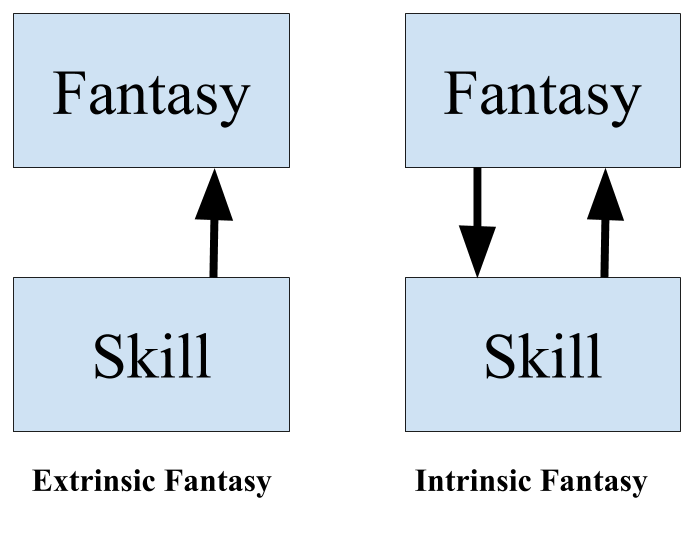
\includegraphics[width=0.6\textwidth]{Images/Theory/SkillFantasy.png}
    \centering
    \caption{Logical dependencies in extrinsic and intrinsic fantasies \citep{malone_what_1980}.}
    \label{fig:skill_fantasy}
    \vspace*{-0.5\baselineskip}
\end{figure}

Fantasies that have a two-way logical dependency are named intrinsic fantasies; the fantasy depends on the skill, and the skill depends on the fantasy. Figure \ref{fig:skill_fantasy} illustrates the two types of fantasy side-by-side. In the spelling game Hangman, the player’s spelling skills affect the fantasy, and the feedback of right or wrong guesses from the fantasy influences the player's skill as it becomes easier to guess new letters each time.

\textbf{The emotional aspect of fantasy} \\
Fantasies in games can appeal to players differently based on what emotions they need to satisfy \citep{malone_what_1980}. It may be challenging to design a computer game that meets the emotional needs of the person playing. Malone states that “... fantasies can be very important in creating intrinsically motivating environments but that, unless the fantasies are carefully chosen to appeal to the target audience, they may actually make the environment less interesting rather than more.” \citep{malone_heuristics_1982}. This statement suggests that different people find different fantasies appealing and that the fantasy must be appropriate for the target audience. Furthermore, if games had different fantasies to choose between, players are more likely to find it enjoyable, motivating, and engaging because it has a broader appeal.

\subsubsection{Curiosity}
The last property, curiosity, is about a player’s motivation to learn within a game environment. The learning is, however, independent from goal-seeking or fantasy-fulfillment. Games can trigger a player's curiosity by creating optimal information complexity environments based on their existing knowledge. Finding such balance for the information complexity will evoke the player’s curiosity to explore the environment further. An optimal environment has a complexity level where the player uses its knowledge to create an expectation of how the environment should behave. Still, these expectations should sometimes be unmet to be novel and introduce an element of surprise. Malone states curiosity should be distinguished into two categories: sensory and cognitive.

\textbf{Sensory curiosity} \\
Sensory curiosity is about the use of sensory-stimulating technology that attracts the user’s attention. In games, sensory curiosity appears as both audio or visual effects. Malone suggests that the effects can be used in four main ways \citep{malone_what_1980}:

\begin{enumerate}
    \item \textbf{As decoration} \\
    The use of audio and visual effects that are present regardless of user interactions. In games like Just Dance Now, this can be found as background music in the menu.
    \item \textbf{For enhancing fantasy} \\
    Sensory curiosity is used to improve fantasy in a game like “decorative” effects. However, the special effects are distinguishable because of their captivating nature and association with fantasy. In Wii Fit, this appears as audio effects that mimic an audience.
    \item \textbf{As a reward} \\
    The use of audio and graphical effects to reward good performance. It can increase the motivation for reaching the goal. Pokémon Go uses flashing lights and stars, together with victory sound, when users perform well, for instance, when they catch a new Pokémon.
    \item \textbf{As a representation system} \\
    Is the use of audio and visuals to convey information without using text. This usage is widely used in games to share information with the user efficiently. If a player in Pokémon Go unsuccessfully throws a Pokéball at a Pokémon, then the Pokéball will bounce away to indicate that a player missed the Pokémon.
\end{enumerate}

\textbf{Cognitive curiosity} \\
Cognitive curiosity is about the desire to improve one’s knowledge structures. Malone claims that people prefer their cognitive structures to be complete, consistent, and parsimonious. According to his theory, to stimulate a player’s cognitive curiosity, they must be given just enough information to make their existing knowledge appear incomplete, inconsistent, or miserly. Cognitive curiosity will engage the user because people are willing to learn more to improve their knowledge-structures. A typical example occurs when people are watching a movie with only some minutes left. The probability of them watching the rest of the video is high because they want to figure out how it will end and bring completeness to their knowledge structure.

\subsection{The GameFlow Framework}
Another essential framework for creating good games is \citeauthor{sweetser_gameflow_2005}’s “GameFlow: A Model for Evaluating Player Enjoyment in Games“ from \citeyear{sweetser_gameflow_2005}. The authors define a model for designing, evaluating, and understanding enjoyment in games based on work previously done by \citeauthor{csikszentmihalyi_flow_1990} in 1990. \citeauthor{csikszentmihalyi_flow_1990} conducted extensive research and surveys to find out what makes experiences enjoyable. Sweetser and Wyeth modified these principles to be representative of enjoyment in games. The GameFlow model consists of eight elements—concentration, challenge, skills, control, clear goals, feedback, immersion, and social interaction. Each of these includes a goal and a set of criteria that can be used when developing games \citep{sweetser_gameflow_2005}.

\subsubsection{Concentration}
Concentration is the first of the eight elements presented in the article. Enhancing how much concentration a task requires increases its immersion. Games should grab the player’s attention immediately and keep holding it for as long as possible. The player’s workload should be maintained at an appropriate level, and unimportant tasks should not be presented during the game to achieve this. Also, nongame-related interactions (e.g., settings menu) should be minimized, and the game should strive to use as much screen real estate  as possible for the gameplay. 

In Guitar Hero, players have to stay highly concentrated throughout the game. The gameplay is set in an environment with few distractions so that the player can become more immersed. The game also forces the player to stay concentrated throughout the song to avoid ending up in the game-over state. Figure \ref{fig:guitar_hero_gameplay} illustrates a screenshot from the gameplay in Guitar Hero.

\begin{figure}[H]
    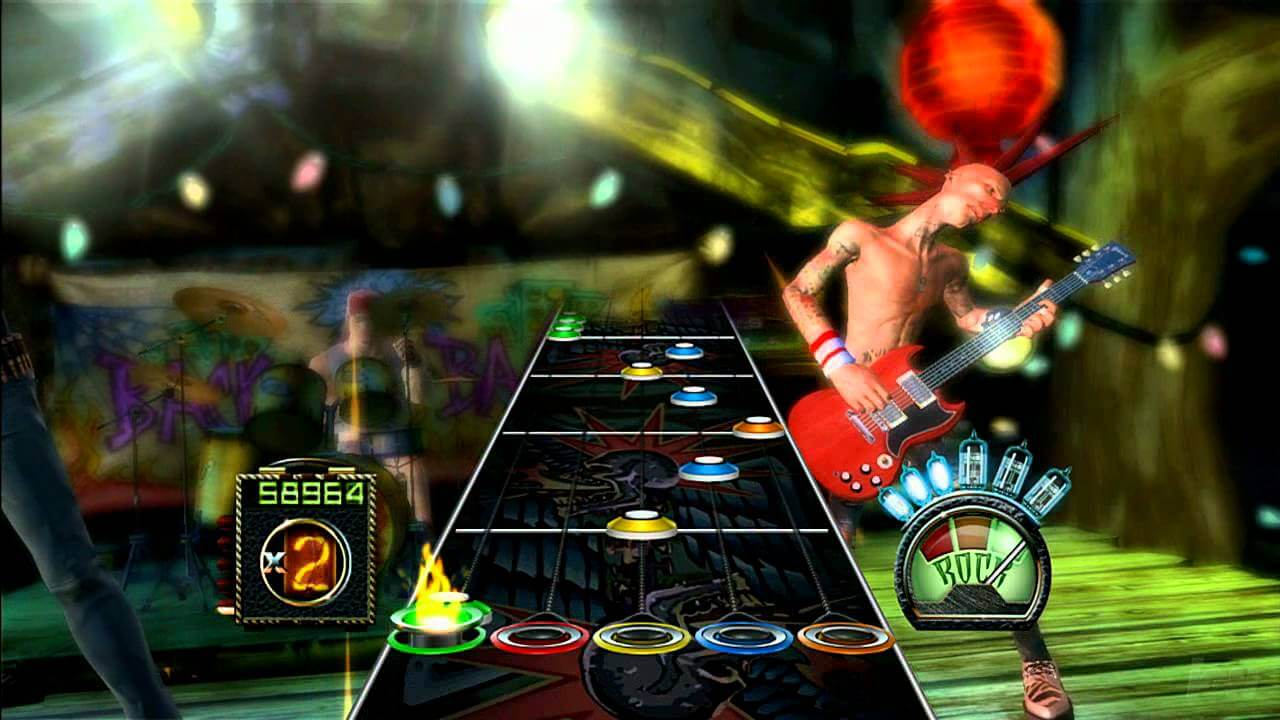
\includegraphics[width=0.85\textwidth]{Images/Theory/GuitarHeroGameplay.jpg}
    \centering
    \caption{Screenshot of gameplay in Guitar Hero.}
    \label{fig:guitar_hero_gameplay}
    \vspace*{-0.5\baselineskip}
\end{figure}

\subsubsection{Challenge}
Challenge is often considered the essential aspect of good game design, and appropriate challenges should be presented to the player. The players’ skill levels should match the challenges given. Additionally, the challenge level should increase as the player moves through the game at an appropriate pace. In the language learning game Duolingo, players take a placement test to start at a proper level of challenge, as seen in Figure \ref{fig:dulingo_placement_test}. This test makes sure that any previous language experience is considered to match the player’s skill to the level of difficulty.

\begin{figure}[H]
    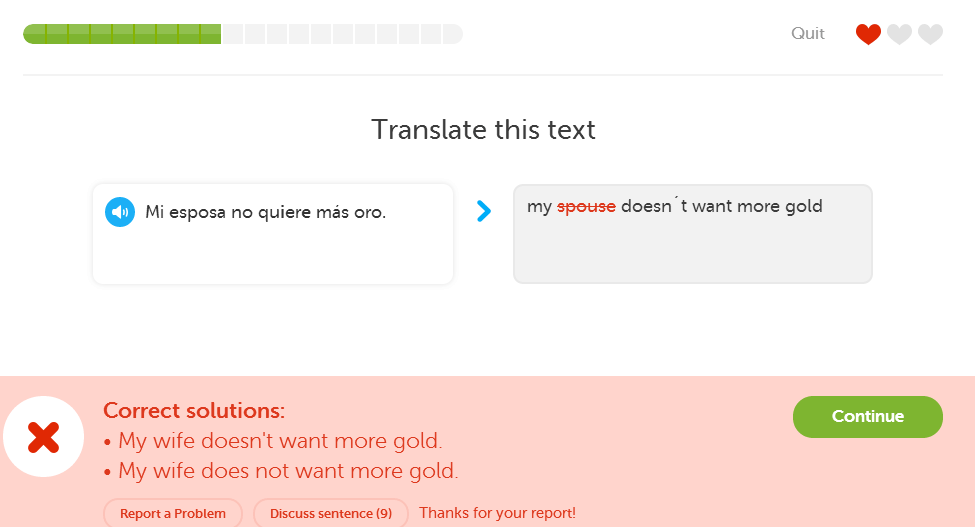
\includegraphics[width=0.85\textwidth]{Images/Theory/DuolingoPlacementTest.png}
    \centering
    \caption{Spanish placement test in Duolingo.}
    \label{fig:dulingo_placement_test}
    \vspace*{-0.5\baselineskip}
\end{figure}

\subsubsection{Player Skills}
As mentioned above, the player’s skill level needs to match the difficulty level of the game. The player’s skills also need to increase during the game, at the same rate as the difficulty of challenges. If not, the game could quickly get too challenging or too easy. Rewarding players appropriately when completing specific tasks, with points or similar, is an essential part of this process.

Again, in Duolingo, players are matched with the appropriate skill level, and as the game progresses, both the player’s skills and the level of difficulty grows. The placement test, see Figure \ref{fig:dulingo_placement_test}, makes sure that players are met with an appropriate level of difficulty. Also, players have to put their knowledge to the test before they are allowed to ascend to the next level. This additional test mechanism makes sure that users are qualified for new levels and prevents players from being demotivated from challenges that are too demanding.

\subsubsection{Control}
Another central element of good game design is control. The players should feel a sense of control over their actions in the game and transfer their intentions to in-game behavior. Essential aspects of the game to achieve this are intuitive interfaces and easy-to-use input devices. Controlling the game should be intuitive and straightforward. In addition to this, players should not make errors that are disturbing to the gameplay. If they do, recovering from their mistakes should be supported. 

Racing games are, in general, examples of games that are intuitive to maneuver. Custom racing wheel controllers mimic the action of actually driving a car, as seen in Figure \ref{fig:racing_wheel_controller}. Recovering from errors that are disturbing for the gameplay, such as flipping the car or driving off a cliff, is also usually supported with a “reset” button.

\begin{figure}[H]
    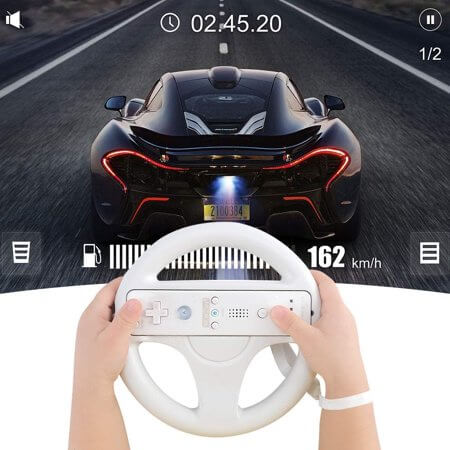
\includegraphics[width=0.6\textwidth]{Images/Theory/wii_racing_wheel_control.jpeg}
    \centering
    \caption{Wii Steering wheel used to play a racing game.}
    \label{fig:racing_wheel_controller}
    \vspace*{-0.5\baselineskip}
\end{figure}

\subsubsection{Clear Goals}
Clear goals should be provided to the user at appropriate times. A primary goal should initially be presented to the user. Some introductory cinematic history that tells the story’s background is often used to describe this goal to the user. Intermediary goals should be provided to the user when they progress. Games often use “briefings” or “missions” for this. 

In Super Mario Bros, players are introduced to a mission of saving Princess Peach from the villain Bowser. This background establishes a clear goal for the entire game. The game also has intermediate objects of completing each level towards the final goal.

\subsubsection{Immersion}
Immersion describes a deep and effortless involvement in games. Players should feel engaged by the game to experience an altered sense of time, less awareness of surroundings, less self-awareness, and fewer worries. Immersion also indicates emotional attachment to the game. Examples of game elements that can increase immersion are audio and narratives. Sounds and music in games improve the players’ attraction to the game and keep them immersed for a more extended period. A history that gives the player some background information or a storyline also creates the same effect.

The role-playing game the Witcher 3 has become known for being a highly immersive open-world game. The game has a strong storyline, realistic graphics and audio, and many intermediate goals that draw the player deeper into the game, as seen in Figure \ref{fig:witcher3_immersion}. For Witcher 3, immersion can cause players to feel an emotional attachment to the game and reduced concern for self and sense of time.

\begin{figure}[H]
    \vspace*{0.5\baselineskip}
    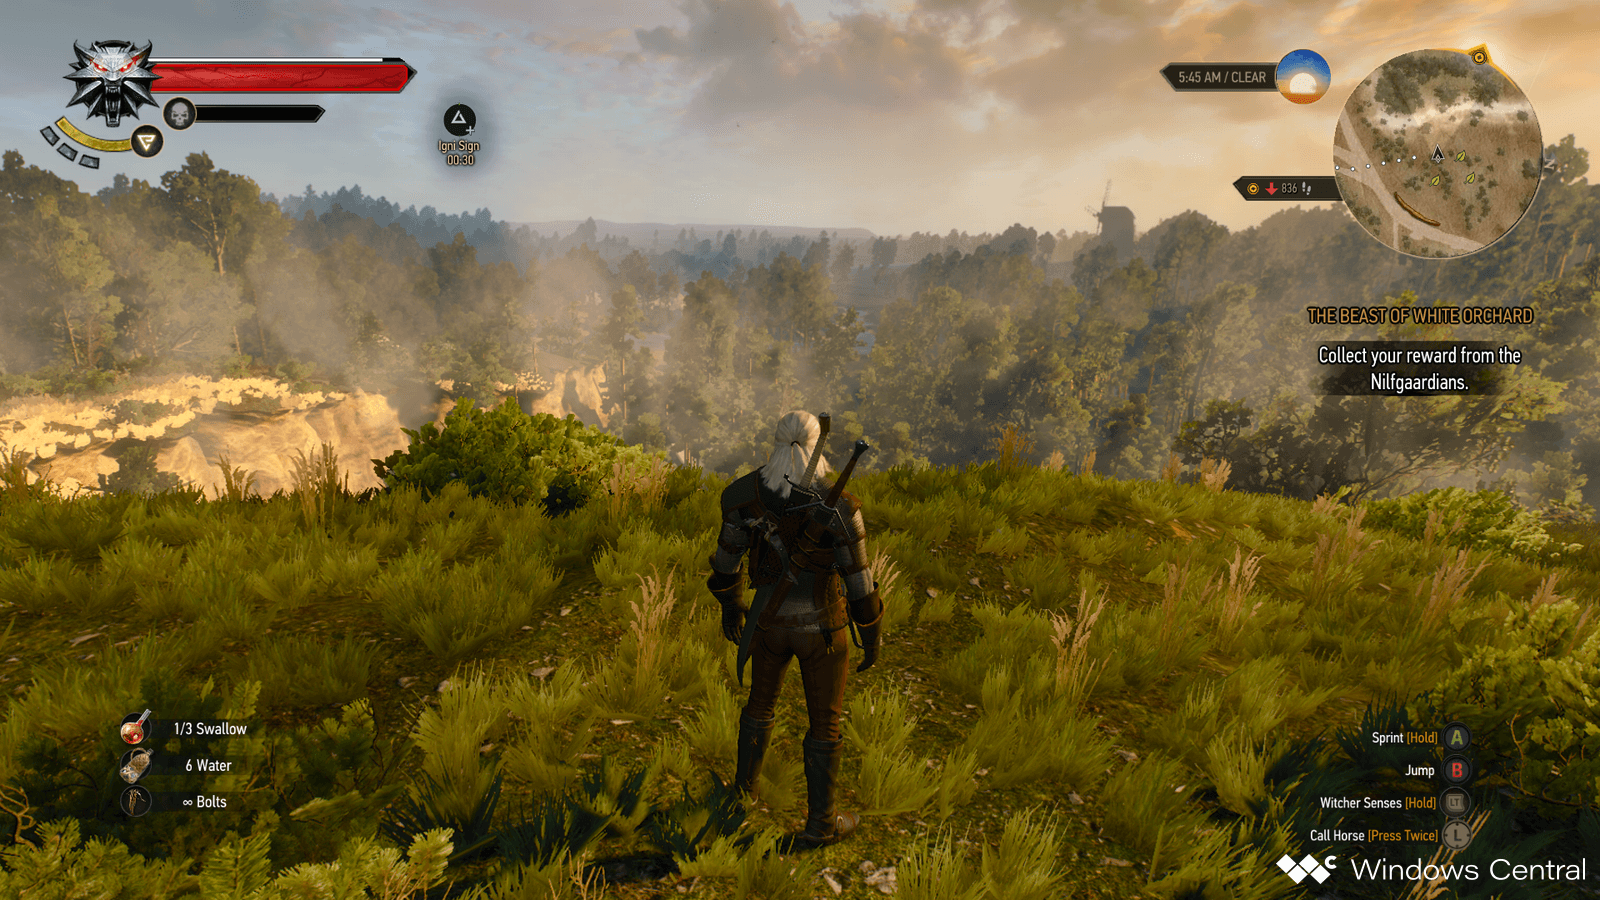
\includegraphics[width=0.85\textwidth]{Images/Theory/witcher3_immersion.png}
    \centering
    \caption{Screenshot from gameplay in Witcher 3.}
    \label{fig:witcher3_immersion}
    \vspace*{2\baselineskip}
\end{figure}

\subsubsection{Feedback}
\begin{wrapfigure}{r}{0.45\textwidth}
    \centering
    \vspace*{-1.5\baselineskip}
    
\includegraphics[width=0.35\textwidth]{Images/Theory/PokemonGoLevelUp.jpg}
    \caption{Feedback in Pokémon Go when leveling up.}
    \vspace*{-\baselineskip}
    \label{fig:pokemon_go_level_up}
\end{wrapfigure}
Players should get the feedback they need during the game. They should always know their status or score and progress towards the goal. Additionally, appropriate feedback based on their actions should be provided.

Pokémon Go uses direct and immediate feedback. Visual, textual, and audio feedback is used frequently. The game also uses points, levels, streaks, and medals to award good performance and engagement. Figure \ref{fig:pokemon_go_level_up} shows the visual feedback a player receives when leveling up in Pokémon Go.

\subsubsection{Social Interaction}
The last element in the GameFlow model is not an element of flow. Social interaction may often interrupt the immersion in games. However, it is an essential element in the GameFlow model because social interactions improve enjoyment in games. Games should support and create opportunities for player-to-player communication and social competitions. Online games are a typical example of how important social interaction can be. In this type of game, social interaction is often the main reason people are attracted to them. World of Warcraft is a classic example of such a game. 

Another example is social motives like affiliation and recognition in online fitness communities (OFC). A 2018 study on running motivations concluded OFC users are significantly more oriented towards achieving running goals and entering competitions than non-OFC users \citep{stragier_recreational_2018}. The results suggest that social gamification features such as recognition or leaderboards in these communities affect player motivation and enjoyment.

\subsection{Summary}
In this chapter, two frameworks describing how to create an enjoyable game have been presented. The frameworks include a description of central elements in game-design associated with producing good games. Even though all framework characteristics are essential aspects, a game should not necessarily incorporate all of them. As a game designer, the most valuable knowledge is understanding the theory and utilizing the appropriate parts.

The concept and elements proposed by \citeauthor{malone_what_1980} and \citeauthor{sweetser_gameflow_2005} will help invent new alternative games and develop our chosen concept later in this thesis. As described in the motivation (Chapter \ref{chap:motivation}), our focus is to create a socially beneficial alternative game. Consequently, the social element in the GameFlow model will be the essential consideration that should influence our game design. However, the other elements will also serve as guidelines and inspiration for us when developing the game. To what extent and which parts are used to create our game will be described later.
